\documentclass[10pt,a4paper,onecolumn]{article}
% \usepackage[utf8]{inputenc}
\usepackage{marginnote}
\usepackage{graphicx}
\usepackage{xcolor}
\usepackage{authblk,etoolbox}
\usepackage{titlesec}
\usepackage{calc}
\usepackage{hyperref}
\hypersetup{breaklinks=true,
            bookmarks=true,
            pdfauthor=
{
      Mario Senden,
      Jannis Schuecker,,
      Jan Hahne,,
      Markus Diesmann,,
      Rainer Goebel,,
  },
            pdftitle=
{
[Re] A neural model of the saccade generator in the reticular formation
},
            colorlinks=true,
            citecolor=blue,
            urlcolor=blue,
            linkcolor=blue,
            pdfborder={0 0 0}}
\urlstyle{same}
\usepackage{tcolorbox}
\usepackage{ragged2e}
\usepackage{fontspec}
\usepackage{fontawesome}
\usepackage{caption}
\usepackage{listings}
\lstnewenvironment{code}{\lstset{language=Haskell,basicstyle=\small\ttfamily}}{}



%\usepackage{fancyvrb}
%\VerbatimFootnotes
%\usepackage{graphicx}
%\usepackage{mdframed}
%\newmdenv[backgroundcolor=lightgray]{Shaded}


\usepackage{longtable,booktabs}

\usepackage[
  backend=biber,
%  style=alphabetic,
%  citestyle=numeric
]{biblatex}
\bibliography{senden-schuecker-hahne-diesmann-goebel-2017.bib}



% --- Macros ------------------------------------------------------------------
\renewcommand*{\bibfont}{\small \sffamily}

\definecolor{red}{HTML}{CF232B}
\newcommand{\ReScience}{Re{\bfseries \textcolor{red}{Science}}}

\newtcolorbox{rebox}
   {colback=blue!5!white, colframe=blue!40!white,
     boxrule=0.5pt, arc=2pt, fonttitle=\sffamily\scshape\bfseries,
     left=6pt, right=20pt, top=6pt, bottom=6pt}

\newtcolorbox{repobox}
   {colback=red, colframe=red!75!black,
     boxrule=0.5pt, arc=2pt, left=6pt, right=6pt, top=3pt, bottom=3pt}

% fix for pandoc 1.14     
\newcommand{\tightlist}{%
  \setlength{\itemsep}{1pt}\setlength{\parskip}{0pt}\setlength{\parsep}{0pt}}

% --- Style -------------------------------------------------------------------
\renewcommand*{\bibfont}{\small \sffamily}
\renewcommand{\captionfont}{\small\sffamily}
\renewcommand{\captionlabelfont}{\bfseries}

\makeatletter
\renewcommand\@biblabel[1]{{\bf #1.}}
\makeatother

% --- Page layout -------------------------------------------------------------
\usepackage[top=3.5cm, bottom=3cm, right=1.5cm, left=1.5cm,
            headheight=2.2cm, reversemp, includemp, marginparwidth=4.5cm]{geometry}

% --- Section/SubSection/SubSubSection ----------------------------------------
\titleformat{\section}
  {\normalfont\sffamily\Large\bfseries}
  {}{0pt}{}
\titleformat{\subsection}
  {\normalfont\sffamily\large\bfseries}
  {}{0pt}{}
\titleformat{\subsubsection}
  {\normalfont\sffamily\bfseries}
  {}{0pt}{}
\titleformat*{\paragraph}
  {\sffamily\normalsize}


% --- Header / Footer ---------------------------------------------------------
\usepackage{fancyhdr}
\pagestyle{fancy}
%\renewcommand{\headrulewidth}{0.50pt}
\renewcommand{\headrulewidth}{0pt}
\fancyhead[L]{\hspace{-1cm}\includegraphics[width=4.0cm]{rescience-logo.pdf}}
\fancyhead[C]{}
\fancyhead[R]{} 
\renewcommand{\footrulewidth}{0.25pt}

\fancyfoot[L]{\hypersetup{urlcolor=red}
              \sffamily \ReScience~$\vert$
              \href{http://rescience.github.io}{rescience.github.io}
              \hypersetup{urlcolor=blue}}
\fancyfoot[C]{\sffamily \thepage}
\fancyfoot[R]{\sffamily Month 2017 $\vert$
                        Volume \textbf{1} $\vert$
                        Issue \textbf{1}}
\pagestyle{fancy}
\makeatletter
\let\ps@plain\ps@fancy
\fancyheadoffset[L]{4.5cm}
\fancyfootoffset[L]{4.5cm}

% --- Title / Authors ---------------------------------------------------------
% patch \maketitle so that it doesn't center
\patchcmd{\@maketitle}{center}{flushleft}{}{}
\patchcmd{\@maketitle}{center}{flushleft}{}{}
% patch \maketitle so that the font size for the title is normal
\patchcmd{\@maketitle}{\LARGE}{\LARGE\sffamily}{}{}
% patch the patch by authblk so that the author block is flush left
\def\maketitle{{%
  \renewenvironment{tabular}[2][]
    {\begin{flushleft}}
    {\end{flushleft}}
  \AB@maketitle}}
\makeatletter
\renewcommand\AB@affilsepx{ \protect\Affilfont}
%\renewcommand\AB@affilnote[1]{{\bfseries #1}\hspace{2pt}}
\renewcommand\AB@affilnote[1]{{\bfseries #1}\hspace{3pt}}
\makeatother
\renewcommand\Authfont{\sffamily\bfseries}
\renewcommand\Affilfont{\sffamily\small\mdseries}
\setlength{\affilsep}{1em}

\LetLtxMacro{\OldIncludegraphics}{\includegraphics}
\renewcommand{\includegraphics}[2][]{\OldIncludegraphics[width=12cm, #1]{#2}}


% --- Document ----------------------------------------------------------------
\title{[Re] A neural model of the saccade generator in the reticular formation}

    \usepackage{authblk}
                        \author[1, 2]{Mario Senden}
                    \author[3]{Jannis Schuecker,}
                    \author[4]{Jan Hahne,}
                    \author[3, 5, 6]{Markus Diesmann,}
                    \author[1, 2, 7]{Rainer Goebel,}
                            \affil[1]{Department of Cognitive Neuroscience, Faculty of Psychology and
Neuroscience, Maastricht University, 6201BC Maastricht, The Netherlands}
                    \affil[2]{Maastricht Brain Imaging Centre, Faculty of Psychology and Neuroscience,
Maastricht University, P.O. Box 616, 6200 MD Maastricht, The Netherlands}
                    \affil[3]{Institute of Neuroscience and Medicine (INM-6) and Institute for
Advanced Simulation (IAS-6) and JARA BRAIN Institute I, Jülich Research
Centre, 52428 Jülich, Germany}
                    \affil[4]{School of Mathematics and Natural Sciences, Bergische Universit"at
Wuppertal, Wuppertal, Germany}
                    \affil[5]{Department of Psychiatry, Psychotherapy and Psychosomatics, Medical
Faculty, RWTH Aachen University, 52062 Aachen, Germany}
                    \affil[6]{Department of Physics, Faculty 1, RWTH Aachen University, 52062 Aachen,
Germany}
                    \affil[7]{Department of Neuroimaging and Neuromodeling, Netherlands Institute for
Neuroscience, an Institute of the Royal Netherlands Academy of Arts and
Sciences (KNAW), 1105BA Amsterdam, The Netherlands}
            
\date{\vspace{-5mm}
      \sffamily \small \href{mailto:mario.senden@maastrichtuniversity.nl}{mario.senden@maastrichtuniversity.nl}}


\setlength\LTleft{0pt}
\setlength\LTright{0pt}


\begin{document}
\maketitle

\marginpar{
  %\hrule
  \sffamily\small
  %\vspace{2mm}
  {\bfseries Editor}\\
  Name Surname\\

  {\bfseries Reviewers}\\
        Name Surname\\
        Name Surname\\
  
  {\bfseries Received}  Month, Day, 2017\\
  {\bfseries Accepted}  Month, Day, 2017\\
  {\bfseries Published} Month, Day, 2017\\

  {\bfseries Licence}   \href{http://creativecommons.org/licenses/by/4.0/}{CC-BY}

  \begin{flushleft}
  {\bfseries Competing Interests:}\\
  The authors have declared that no competing interests exist.
  \end{flushleft}

  \hrule
  \vspace{3mm}

  \hypersetup{urlcolor=white}
  
    \vspace{-1mm}
  \begin{repobox}
    \bfseries\normalsize
      \href{http://github.com/rescience/rescience-submission/article}{\faGithubAlt~Article repository}
  \end{repobox}
      \vspace{-1mm}
  \begin{repobox}
    \bfseries\normalsize
      \href{http://github.com/rescience/rescience-submission/code}{\faGithubAlt~Code repository}
  \end{repobox}
        \hypersetup{urlcolor=blue}
}

\begin{rebox}
\sffamily {\bfseries A reference implementation of}
\small
\begin{flushleft}
\begin{itemize}
    \item[→] \emph{A neural model of the saccade generator in the reticular
formation}, G. Gancarz, S. Grossberg, Neural Networks, 1159-1174, 1998
  \end{itemize}\par
\end{flushleft}
\end{rebox}


\section{Introduction}\label{introduction}

We provide an implementation of the saccade generator (SG); a rate
neuron model of the neural circuitry in the reticular formation proposed
by Gancarz \& Grossberg \autocite{Gancarz1998}. The same group has
recently sucessfully embedded the SG into a larger model of the eye
movement network \autocite{Grossberg2012} showcasing its compatible
nature. This compatibility of the SG model might prove useful in the
future for studying the interplay of neural (sub)systems of visuo-motor
integration. It is thus of interest to implement the model in publicly
available, widely used, and actively developed neural simulation
frameworks such as NEST \autocite{Gewaltig2007}. We show that the model
translates well to the NEST framework as our implementation faithfully
reproduces most simulation results reported in the original publication.
Our code uses the Python interface \autocite{Eppler2008} for legibility
with both model and analysis scripts being implemented using Python
2.7.12.

\section{Methods}\label{methods}

We largely follow the descriptions of the model provided in the original
publication with a number well-motivated exceptions. First, in the
original description, neuron activations are bounded from below at zero
resulting in their rectification at every step in the numerical
integration. Since this effectively alters neuron dynamics from their
original description, we refrained from this practice. Instead, input
received by each neuron from other neurons was passed through a
rectified linear gain function before summation. This assured that
neuron dynamics accorded with their description. Second, the gain
function \[ g(x) = {\frac{x^4}{0.1^4+x^4}} \] \{\#eq:1\} (equation A11)
in the original publication was replaced by
\[ g(x) = {\frac{1}{e^{-40(x-0.1)}}} \] \{\#eq:2\} to prevent positive
responses to negative net input but otherwise preserve the shape of the
curve for \(\mathrm{x>0}\). Third, according to equation A12 in the
original publication horizontal eye position \(\theta\) is given by
\(\mathrm{\theta=260({TN}_{r}-0.5)}\). However, activation of tonic
neurons (TNs) is 0 rather than 0.5 when the eye is at the center of its
range and a factor of 260 produces saccades of excessively high
amplitudes. We found a factor of 150 to reproduce original simulations
better. Finally, the original implementation uses the fourth order
Runge--Kutta method for numerical integration. Instead, we used the
Exponential Euler method which is standardly implemented in NEST for the
numerical integration of rate neurons \autocite{Hahne2016}.

In addition to these changes, the original model description has two
features which cannot be straightforwardly translated to NEST. First,
whether a nonlinear gain function is applied to a neuron's input can
depend on the origin of said input. This is notably the case for
excitatory burst neurons (EBNs) and omnipause neurons (OPNs). Since NEST
only applies a single gain function per neuron to each of its input, we
opted for using a linear gain function for EBNs and OPNs and to pass
those inputs requiring an additional nonlinear gain function through an
auxiliary unit instantaneously applying the desired nonlinearity.
Second, constant input to a neuron was provided by an appropriately
weighted bias node.

\section{Results}\label{results}

In the remainder we present the results of our simulations for all nine
experiments reported in the original publication. While our results
generally accord very well with those of Gancarz \& Grossberg
\autocite{Gancarz1998}, some simulations required slightly divergent
parameter values to reproduce original results.

\subsection{1) Saccadic staircase
simulation}\label{saccadic-staircase-simulation}

The first simulation reported by Gancarz \& Grossberg
\autocite{Gancarz1998} showcases the evolution of activity for each
neuron type in the horizontal SG to a constant input (\(\mathrm{I=1}\))
applied to the left long-lead burst neuron (LLBN) for
\(265\,\mathrm{ms}\).

\begin{figure}
\centering
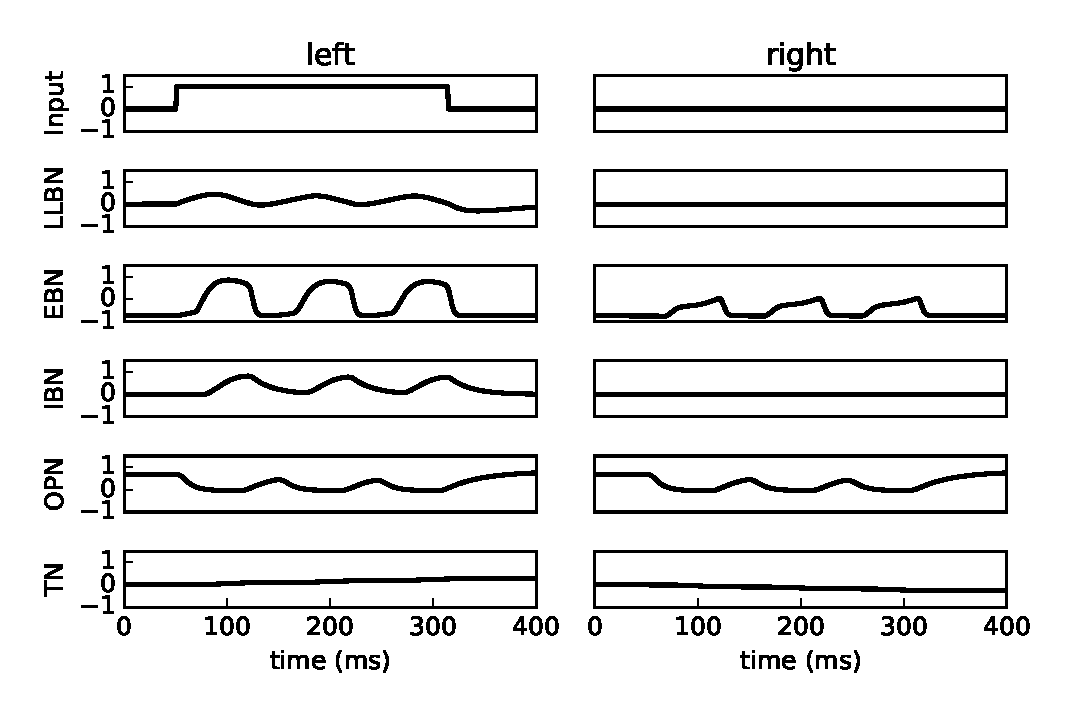
\includegraphics{../code/fig3.eps}
\caption{\textbf{Figure caption for part (A) and part (B) .} Description
of stuff happening in the original implementation of Gancarz \&
Grossberg \autocite{Gancarz1998}.}\label{fig:fig_1}
\end{figure}

\subsection{Cell activity profiles in the reticular
formation}\label{cell-activity-profiles-in-the-reticular-formation}

blubber

\begin{figure}
\centering
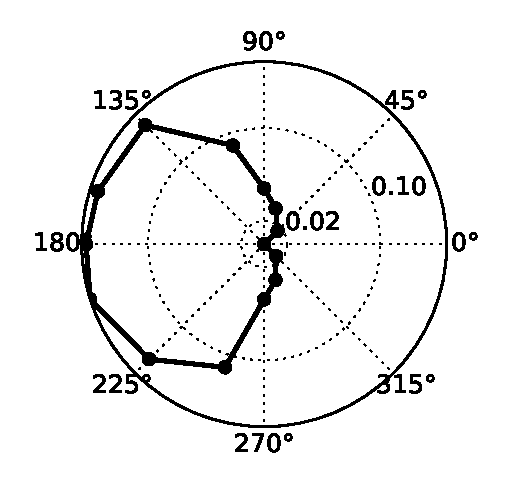
\includegraphics[width=6.37500cm,height=8.50000cm]{../code/fig5.eps}
\caption{\textbf{Figure caption for part (A) and part (B) .} Description
of stuff happening in the original implementation of Gancarz \&
Grossberg \autocite{Gancarz1998}.}\label{fig:fig_2}
\end{figure}

\subsection{Visually guided saccades}\label{visually-guided-saccades}

Bli Bla Blub

\begin{figure}
\centering
\includegraphics[width=8.50000cm,height=8.50000cm]{../code/fig6.eps}
\caption{\textbf{Figure caption for part (A) and part (B) .} Description
of stuff happening in the original implementation of Gancarz \&
Grossberg \autocite{Gancarz1998}.}\label{fig:fig_3}
\end{figure}

\subsection{Oblique staircase
simulation}\label{oblique-staircase-simulation}

Bli Bla Blub

\begin{figure}
\centering
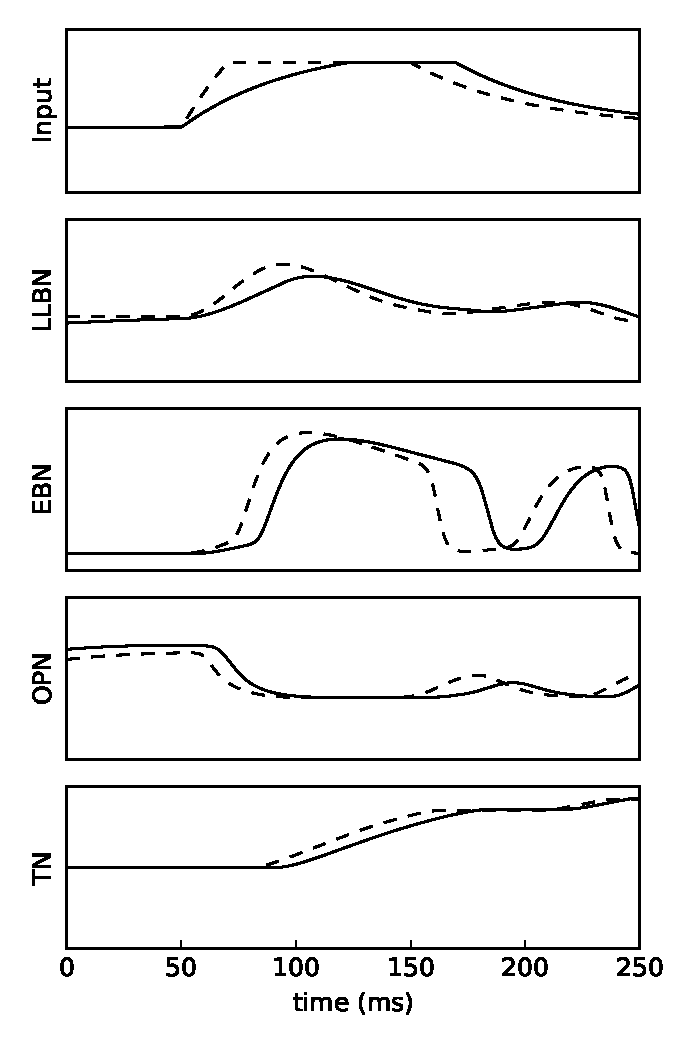
\includegraphics[width=8.50000cm,height=11.60000cm]{../code/fig7.eps}
\caption{\textbf{Figure caption for part (A) and part (B) .} Description
of stuff happening in the original implementation of Gancarz \&
Grossberg \autocite{Gancarz1998}.}\label{fig:fig_4}
\end{figure}

\subsection{Tuning curve of excitatory burst neuron
(EBN)}\label{tuning-curve-of-excitatory-burst-neuron-ebn}

Bli Bla Blub

\begin{figure}
\centering
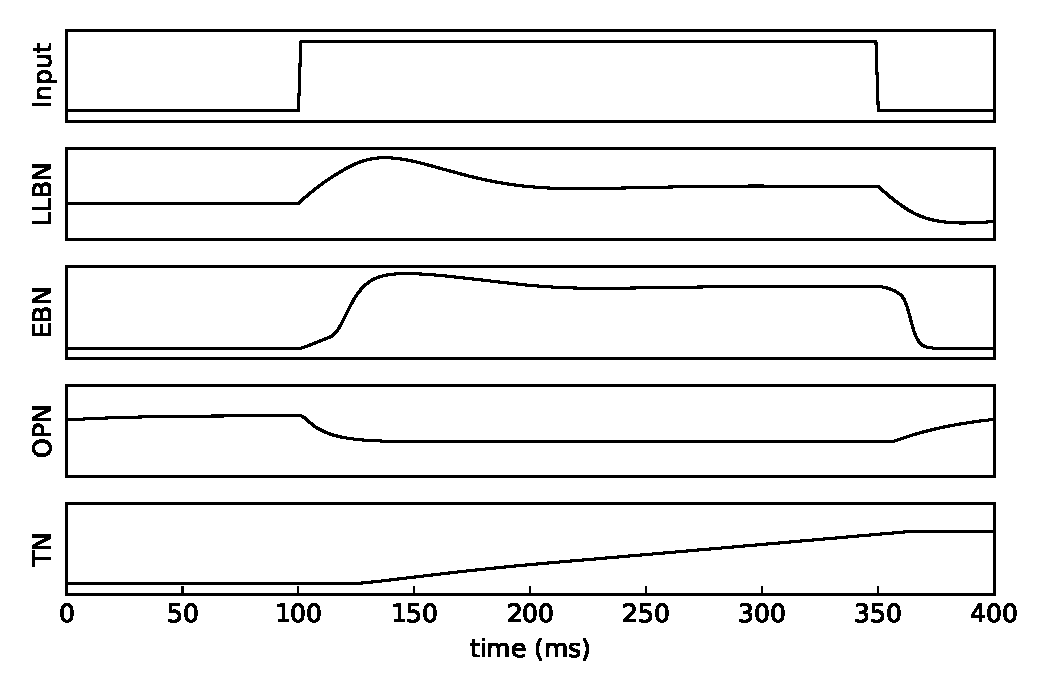
\includegraphics[width=8.50000cm,height=8.50000cm]{../code/fig8.eps}
\caption{\textbf{Figure caption for part (A) and part (B) .} Description
of stuff happening in the original implementation of Gancarz \&
Grossberg \autocite{Gancarz1998}.}\label{fig:fig_5}
\end{figure}

\subsection{Effects of frequency of external
stimulation}\label{effects-of-frequency-of-external-stimulation}

Bli Bla Blub

\begin{figure}
\centering
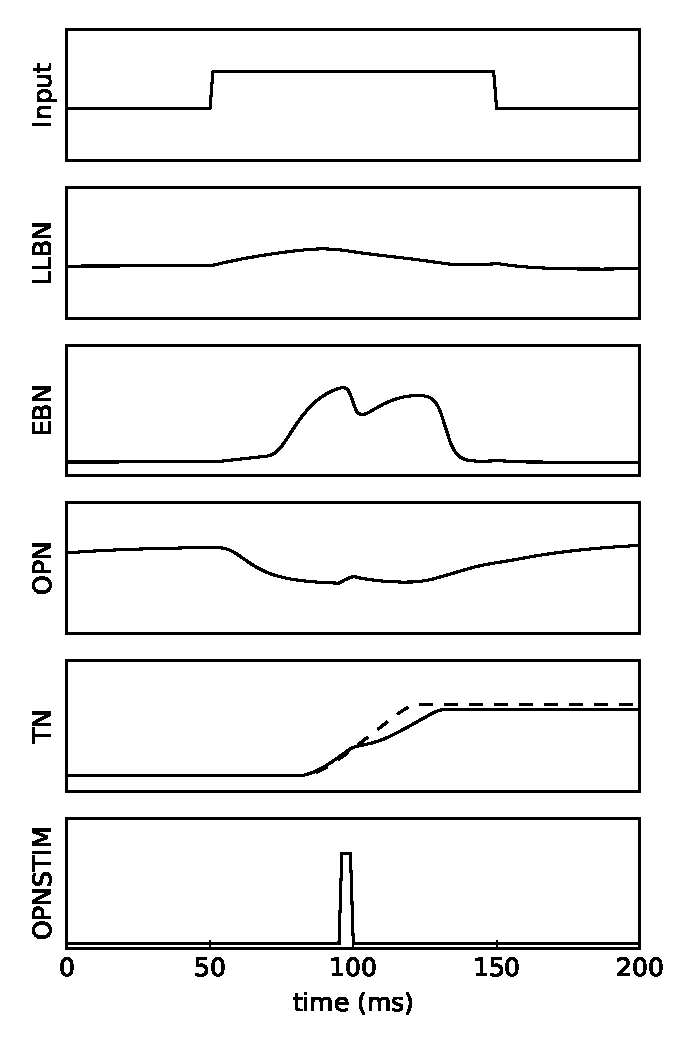
\includegraphics[width=11.60000cm,height=5.00000cm]{../code/fig9.eps}
\caption{\textbf{Figure caption for part (A) and part (B) .} Description
of stuff happening in the original implementation of Gancarz \&
Grossberg \autocite{Gancarz1998}.}\label{fig:fig_6}
\end{figure}

\subsection{Trading saccade velocity and
duration}\label{trading-saccade-velocity-and-duration}

Bli Bla Blub

\begin{figure}
\centering
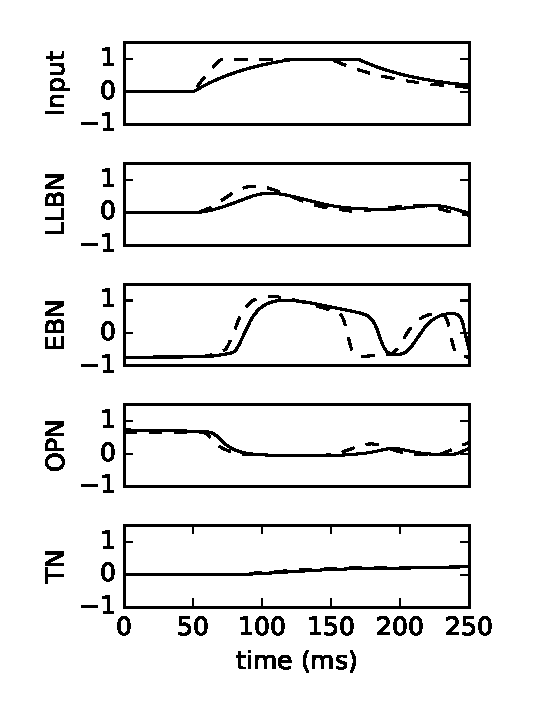
\includegraphics[width=8.50000cm,height=11.60000cm]{../code/fig10.eps}
\caption{\textbf{Figure caption for part (A) and part (B) .} Description
of stuff happening in the original implementation of Gancarz \&
Grossberg \autocite{Gancarz1998}.}\label{fig:fig_7}
\end{figure}

\subsection{Smooth staircase
simulation}\label{smooth-staircase-simulation}

Bli Bla Blub

\begin{figure}
\centering
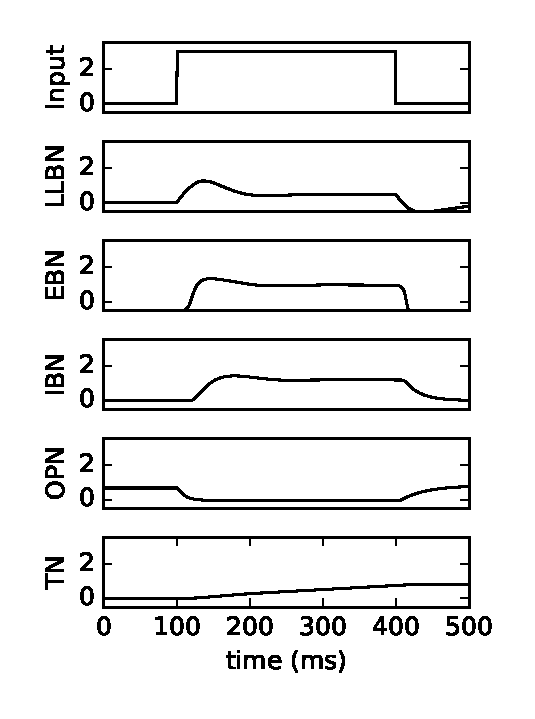
\includegraphics[width=8.50000cm,height=11.60000cm]{../code/fig11.eps}
\caption{\textbf{Figure caption for part (A) and part (B) .} Description
of stuff happening in the original implementation of Gancarz \&
Grossberg \autocite{Gancarz1998}.}\label{fig:fig_8}
\end{figure}

\subsection{Interrupted saccade
simulation}\label{interrupted-saccade-simulation}

Bli Bla Blub

\begin{figure}
\centering
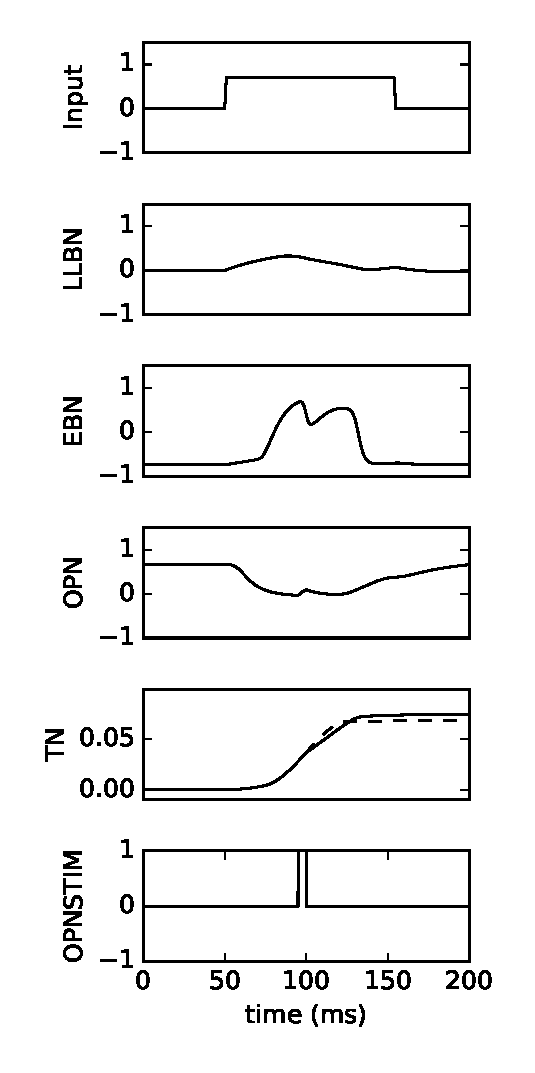
\includegraphics[width=8.50000cm,height=11.60000cm]{../code/fig12.eps}
\caption{\textbf{Figure caption for part (A) and part (B) .} Description
of stuff happening in the original implementation of Gancarz \&
Grossberg \autocite{Gancarz1998}.}\label{fig:fig_9}
\end{figure}

\section{Conclusion}\label{conclusion}

Conclusion, at the very minimum, should indicate very clearly if you
were able to replicate original results. If it was not possible but you
found the reason why (error in the original results), you should exlain
it.

\begin{longtable}[]{@{}llllll@{}}
\caption{Table caption \{\#tbl:table\}}\tabularnewline
\toprule
Heading 1 & & & Heading 2 & &\tabularnewline
\midrule
\endfirsthead
\toprule
Heading 1 & & & Heading 2 & &\tabularnewline
\midrule
\endhead
cell1 row1 & cell2 row 1 & cell3 row 1 & cell4 row 1 & cell5 row 1 &
cell6 row 1\tabularnewline
cell1 row2 & cell2 row 2 & cell3 row 2 & cell4 row 2 & cell5 row 2 &
cell6 row 2\tabularnewline
cell1 row3 & cell2 row 3 & cell3 row 3 & cell4 row 3 & cell5 row 3 &
cell6 row 3\tabularnewline
\bottomrule
\end{longtable}

A reference to table \textcite{tbl:table}. A reference to figure
\textcite{fig:logo}. A reference to equation \textcite{eq:1}. A
reference to citation \textcite{markdown}.

\begin{figure}
\centering
\includegraphics{rescience-logo.pdf}
\caption{Figure caption}\label{fig:logo}
\end{figure}

\[ A = \sqrt{\frac{B}{C}} \] \{\#eq:1\}

\section{Acknowledgments}\label{acknowledgments}

All network simulations carried out with NEST
(http://www.nest-simulator.org).

{\sffamily \small
  \printbibliography[title=References]
}
\end{document}
